\chapter{Young Entrepreneur Interviews Millionaire Justin Waller}

This chapter comes from an interview, not from a formal blackboard lecture, but its inner structure is still quite disciplined. We are led from stakes to method: first the cold-open claims about money, origins, and rebuildability; then the discipline of staying in one fight; then a finite-allocation model of energy; then the arithmetic of starting a business without cash; then the arithmetic of real-estate underwriting; and finally the organizational logic of scaling from seven figures to eight. The mathematics here is therefore not a finished theory written on a board. It is business arithmetic unfolded in the order in which the interview motivates it.

\section{Opening Stakes, Authority, and the Promise of Method}

The source begins with a teaser montage. We are given four forward-facing claims before the interview properly starts: a large annual income, no inherited money, the confidence that everything could be rebuilt if lost, and the question of how one becomes a multimillionaire in the present world. These are not yet explanations. They are promises. They tell us what sort of problem the interview will try to solve.

Only after that does the host reset in Miami and explain why Justin Waller is worth listening to: he is presented as a large construction operator, a recognized entrepreneur, and a man who has scaled in both business and real estate. When the formal interview begins, the first facts are simple but important. Waller says he began in steel at age \(24\), has been in construction for about \(15\) years, and now has more than \(200\) men working coast to coast. Later the teaser line ``five in a year'' is clarified as roughly \(\$5\) million take-home, while the businesses are said to have reached roughly \(\$35\) million in scale.

What matters about this opening is not merely the biography. The interview is establishing the right to speak about leverage, systems, and freedom by first establishing domain depth. Before the lecture asks how wealth is structured, it asks who earned the right to answer.

\section{Staying in One Fight}

The first substantive question concerns industry choice and the importance of becoming a master of one thing rather than hopping from industry to industry. Waller's answer is strikingly precise in structure. People get hit a little in one career, change direction, and then suffer the beginner's licks of the next career. The thing he credits in his younger self is not genius, but endurance: he stayed in the same fight long enough to make substantial money and therefore create freedom.

That order matters. Freedom does not appear at the beginning. It appears as the consequence of concentration.

\subsection{Question \& Answer}

\paragraph{Question.} Why does concentration beat premature diversification?

\paragraph{Answer.} Because the scarce object is not abstract opportunity but effective energy. If we repeatedly reset into novice status, we do not let competence, trust, judgment, or operating leverage compound anywhere. The interview's point is not that branching out is always a mistake. It is that branching before freedom is usually an elegant way of staying weak.

The lecture then compresses this into its first real model. We are told that we only get so much energy in life. We have a cup of water; that cup is our energy; and if we pour it over too many plants, none of them bears fruit. A cautious formalization is
\begin{equation}
\sum_{i=1}^{n} e_i = E,
\end{equation}
where \(E\) is the total energy available and \(e_i\) is the allocation to project \(i\). This notation is editorial rather than spoken, but it captures the logic exactly: all ventures draw from the same finite reservoir.

\begin{figure}[h]
\centering
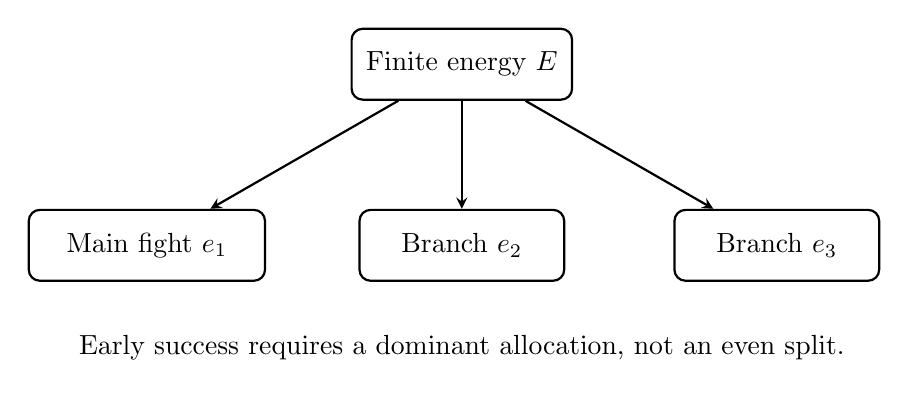
\begin{tikzpicture}[>=stealth, thick]
\node[draw, rounded corners, minimum width=2.8cm, minimum height=0.9cm] (E) at (0,0) {Finite energy \(E\)};
\node[draw, rounded corners, minimum width=3.0cm, minimum height=0.9cm] (p1) at (-4,-2.3) {Main fight \(e_1\)};
\node[draw, rounded corners, minimum width=2.6cm, minimum height=0.9cm] (p2) at (0,-2.3) {Branch \(e_2\)};
\node[draw, rounded corners, minimum width=2.6cm, minimum height=0.9cm] (p3) at (4,-2.3) {Branch \(e_3\)};
\draw[->] (E) -- (p1);
\draw[->] (E) -- (p2);
\draw[->] (E) -- (p3);
\node at (0,-3.6) {Early success requires a dominant allocation, not an even split.};
\end{tikzpicture}
\end{figure}

We should resist the temptation to invent a precise production function. The interview does not give one. But it does give the correct directional claim. In the early phase we do better with
\[
e_1 \gg e_2,e_3,\dots,
\]
than with a flat distribution over many lines of effort. If freedom is first produced in one place, later diversification becomes a consequence of success rather than a substitute for it.

\begin{remark}
This is the first mathematical turn of the lecture. The object being allocated is not capital in the narrow accounting sense, but attention, endurance, and entrepreneurial force.
\end{remark}

\section{No Money, Turning Point, and the Next Mountain}

Only after the concentration argument has been laid down does the interview pivot back to origins. The host asks whether Waller comes from money and then presses further: what was the turning point, and how did seriousness about financial freedom begin? The answer keeps the sequence intact. First there was no money around. Then came the decision not to become the atmosphere in which one had been placed.

\subsection{Question \& Answer}

\paragraph{Question.} What creates the turning point toward financial seriousness?

\paragraph{Answer.} In the logic of the interview, the turning point is not a spreadsheet. It is a refusal. One either becomes the atmosphere one inhabits, or decides to be anything but that atmosphere. From there the motion becomes directional: one finds more consciousness, one climbs one mountain, and then one looks for the next one.

The lecture is careful here. It does not say that wealth comes from resentment alone. It says that dissatisfaction with the given atmosphere starts the motion, but the sustaining principle is still ascent. Happiness, he says, is often on the climbing part, not simply at the peak. This keeps the later arithmetic honest. The financing and leverage sections are not bare techniques detached from motive; they are the next steps after a person has decided what sort of life he refuses to remain in.

\section{Bootstrapping Without Cash}

The source briefly pauses for a promotional interlude and then returns to the interview proper. When it returns, it returns to the most practical question yet: how does a business begin if there is no money to start it? The transcript has a small garble in the lead-in, but the answer itself is perfectly clear. There was no money. Contracts had to be won first. Those contracts then had to be taken to a bank. Only after that could a line of credit be secured.

This is the first point where the interview becomes hard arithmetic. The first credit line is stated explicitly:
\begin{equation}
L_0 = \$15{,}000.
\end{equation}
The payroll is stated explicitly as well:
\begin{equation}
P_{\text{week}} \approx \$2{,}500/\text{week}.
\end{equation}
The setting is correspondingly small: about two men and backyard buildings. The figures are not large, but that is what makes them useful. We can actually see the bridge mechanism.

\subsection{Question \& Answer}

\paragraph{Question.} How do we start when we do not yet have capital?

\paragraph{Answer.} The lecture's answer is not to wait for capital but to manufacture bankable evidence. Contracts come first; bank credit comes second. The entrepreneur does not ask the bank to believe in a dream. He asks the bank to advance against the probability of near-future cash flow.

A first-pass working estimate follows immediately. If we isolate payroll and ignore materials, overhead, and receivables timing, then the credit line implies
\begin{equation}
T_{\text{runway}} \approx \frac{L_0}{P_{\text{week}}}
\approx \frac{15{,}000}{2{,}500}
\approx 6 \text{ weeks}.
\end{equation}
This is not a complete job-cost model. It is a survival estimate. But that is exactly the level at which the lecture wants us to think. The entrepreneur's first mathematics is not elegance. It is the mathematics of not missing payroll.

The causal chain can be written compactly as
\begin{align}
C_{\text{won}}
&\longrightarrow \text{bank evidence}
\longrightarrow L_0
\longrightarrow \text{payroll bridge}.
\end{align}
Here \(C_{\text{won}}\) denotes contracts already won. What matters is the order: win, show, borrow, survive.

We may summarize the spoken mechanism as follows.
\begin{enumerate}
\item Win contracts.
\item Carry those contracts to the bank as evidence.
\item Obtain a line of credit against that evidence.
\item Use the credit line to bridge payroll and early execution until operating cash flow catches up.
\end{enumerate}

The deeper lesson is not merely that debt can be helpful. It is that evidence changes financing terms. Contracts are not just revenue prospects; they are collateral in narrative form.

\section{Real-Estate Underwriting as Practical Arithmetic}

The next technical question asks how leverage capital, good debt, and wealth fit together. This is the chapter's real financial center. Waller says he now owns more than \(400\) doors, that is, more than \(400\) rentable units, and then lists the variables that govern a deal: net operating income, cap rate, debt service, and where we are in the cycle on that property.

The rhetorical force of this section lies in its anti-mystical tone. He does not speak as if real estate were magic. He speaks as if it were arithmetic disciplined by timing.

\subsection{Question \& Answer}

\paragraph{Question.} How do we use leverage without being destroyed by rate risk?

\paragraph{Answer.} We begin by identifying the objects the interview itself names. Let \(\mathrm{NOI}\) be net operating income, let \(V\) denote value or purchase price, and let \(\mathrm{DS}\) denote annual debt service. Then a standard clean notation for two of the central ratios is
\begin{equation}
\mathrm{CapRate} = \frac{\mathrm{NOI}}{V},
\end{equation}
and
\begin{equation}
\mathrm{DSCR} = \frac{\mathrm{NOI}}{\mathrm{DS}}.
\end{equation}
The acronym \(\mathrm{DSCR}\) is editorial, not spoken, but the comparison itself is exactly what the lecture asks us to track: how much income is there, and how heavy is the debt burden imposed upon it?

The interview also describes the capital stack in plain language: other people's money for the down payment and long-term bank debt for the rest. In stripped-down notation,
\begin{equation}
C_{\text{stack}} = E_{\text{outside}} + D_{\text{bank}}.
\end{equation}
This is deliberately minimal. The point is not to import every layer of modern deal finance, but to stay faithful to the lecture's own decomposition.

The real danger arrives through time. Waller imagines a five- to seven-year adjustable-rate mortgage and asks what happens if a loan written in a high-rate world resets into a much harsher one:
\begin{align}
T_{\mathrm{ARM}} &\in [5,7] \text{ years},\\
r_0 &\approx 7.5\%\text{--}8\%, \qquad r_1 \approx 16\%.
\end{align}
The lecture's warning is that, if we do not understand the cycle, we can get to the end of that ARM in an environment that resembles the early 1980s rather than the one we underwrote against.

A cautious stress calculation makes the point. If we temporarily isolate the interest component on balance \(B\), then
\begin{equation}
\mathrm{DS}_{\text{IO}}(r)=rB,
\end{equation}
so that
\begin{equation}
\frac{\mathrm{DS}_{\text{IO}}(0.16)}{\mathrm{DS}_{\text{IO}}(0.08)} = 2.
\end{equation}
This is not a full amortization model. It is only a first sensitivity calculation. But it is enough to show why the lecture insists that the math is simple while the discipline is hard. If the rate component doubles and the income side does not keep pace, then debt service can move from manageable to dangerous rather quickly. In that crude stress frame,
\begin{equation}
\mathrm{DSCR}_{\text{new}}
\approx
\frac{\mathrm{NOI}}{2\,\mathrm{DS}_{\text{old}}}
=
\frac{1}{2}\,\mathrm{DSCR}_{\text{old}},
\end{equation}
again only as a first approximation.

What saves the investor is not formula worship but advance attention. We are told to watch debt service, watch the long-term and short-term debt cycle, and watch where rates may go. The point is to preserve time to act. This is why Waller says the arithmetic is ``third grade math.'' He means that the conceptual burden is not symbolic sophistication. It is disciplined, repeated comparison.

\begin{remark}
The underwriting section should remain close to the interview's own named variables. The source does not present a full spreadsheet, so the notes should not pretend that one was silently present.
\end{remark}

\section{From Assets to Systems}

After the underwriting discussion, the interview broadens briefly into a critique of schooling, a meditation on freedom, and a claim that many people are not living freely enough to say what they actually think. That broader social commentary matters as transition. It prevents the real-estate section from being read as merely technical. The arithmetic, in this lecture, is always tied back to freedom.

The host then returns to scale. The annual money question from the teaser is clarified: roughly \(\$5\) million take-home in a single year, and roughly \(\$35\) million at the business level. The next question is how the move from seven figures to eight figures happens. Here the lecture turns from balance-sheet leverage to human leverage.

Let us name the lecture's four central organizational objects:
\[
S = \text{systems}, \qquad
K = \text{competence}, \qquad
I = \text{intent}, \qquad
O = \text{ownership}.
\]
This is not a literal formula for scale, but it gives us a clean vocabulary for the sequence Waller describes. Systems matter. Competence matters. Intent matters. But even competence and intent are not enough if the people executing the plan have no ownership in the thing being built.

\subsection{Question \& Answer}

\paragraph{Question.} Why do organizations stall when a plan is merely handed down?

\paragraph{Answer.} Because a handed-down plan creates compliance without ownership. In the interview's language, the person sits in the boat with his arms crossed, waiting for it to go wrong. The point is not that staff must formally own equity in every case. The point is that they must be allowed to help build the system they are later asked to run.

The lecture's causal chain is therefore:
\begin{enumerate}
\item choose competent people who can do the work;
\item choose people with intent who want to do the work;
\item let them help build the systems;
\item give them enough autonomy that execution is not passive;
\item align compensation with value creation.
\end{enumerate}

The most revealing sentence in this section is the one about management. We should manage from the standpoint, ``I should be paying you more money,'' not from the standpoint, ``you should be making me richer.'' This is an incentive statement, but it is also a diagnosis of fragility. A firm scales when the person inside it can see his future inside the owner's vision, not when he is merely a reluctant pair of hands.

Thus the lecture gives us a second version of leverage. Earlier we had financial leverage, where outside money and bank debt amplify the return on a property. Here we have organizational leverage, where systems plus capable and invested people amplify the owner's reach. In both cases structure matters more than raw ambition.

\section{Scars, Repetition, and the Rebuild Claim}

The closing movement returns to aphorism, but by now the aphorisms are supported by machinery. Waller's favorite mentor quote is that we can tell the size of a man by the size of his problems. Failures are then recast as the bricks that build the castle. The interview also gives us the phrases ``For every new level, there's a new devil'' and ``Every king's got scars, cowboy.'' These are not detachable slogans pasted onto the end. They are the moral summary of the earlier arithmetic.

The transcript then circles back toward the cold-open challenge. If everything were lost tomorrow, could it all be made back? The answer is yes, and the explanation is again the same one: repetition in one domain becomes a superpower. The follow-up in the closing stretch makes this explicit. If we keep doing the same thing again and again, nobody can take that capacity away. The transcript briefly turns back to steel as the reference domain, which clarifies the earlier colloquial line about being back in six weeks. The real claim is not mystical speed. It is that deep domain competence survives temporary financial destruction.

By the end, then, the opening teaser has been resolved. The lecture has not argued that confidence alone rebuilds wealth. It has argued that repeatable competence, earned by staying in one fight long enough, is the durable asset underneath the cash and the properties.

\section{Summary}

The interview unfolds in a strict order. First it establishes authority and stakes. Then it argues for concentration over premature diversification. Then it translates that claim into a finite-allocation model of entrepreneurial energy. After that it asks how a business begins without money, and answers with contracts, bank evidence, and bridge credit. It then turns to the practical arithmetic of real-estate underwriting: \(\mathrm{NOI}\), cap rate, debt service, capital stack, cycle position, and reset-rate risk. Finally it moves from financial leverage to organizational leverage through systems, competence, intent, ownership, and incentive alignment.

What makes the chapter mathematically interesting is not formal sophistication but disciplined comparison. We compare one industry to many industries, one concentrated allocation to a thin dispersion, payroll to credit, \(\mathrm{NOI}\) to debt service, the initial rate to the reset rate, and the handed-down plan to the co-built system. The lecture insists that wealth-building arithmetic is simple enough to name, but demanding enough to live by. That is why its closing philosophy of scars and repeatability does not sit outside the mathematics. It is the human form of the same principle: what compounds is what survives.